% !TeX spellcheck = es
\documentclass{article}
\usepackage[utf8]{inputenc}
\usepackage{graphicx}
\usepackage{hyperref}
\usepackage{amsmath}
\usepackage{tikz}
\usepackage{float}
\usepackage[simplified]{pgf-umlcd}
\usepackage{subfiles}
\usepackage{listings}
\usepackage[lighttt]{lmodern}
\usepackage{color}
\begin{document}
\section{BiblioCAT}
\subsection{Introducción}
Las libros nos permiten descubrir múndos de fantasia así como entender mejor el mundo en el que vivimos. Nos permiten aprender todo tipo de cosas, desde "Teo va a la escuela" a "Compilers: Principles, Techniques, and Tools".\\\\
%
Las librerias de Cataluña tienen un sistema de intercanvio de libros, de forma que, quando alguien se dirige a una biblioteca a buscar un libro para aprender a programar Haskell, y el/la bibliotecario/a le diga "I eso qué és?!?!?", haya la posibilidad de pedirle a otra biblioteca que tenga el libro que el/la valiente aspirante/a a aprender Haskell pedia.
%
\subsection{Especificaciones}
\begin{itemize}
\item Lo que les gustaria a las bibliotecas és maximizar el tiempo en que los libros estan generando valor, es decir, el tiempo en que un libro esta en manos de algún usuario. \textbf{Cada libro genera un valor X.} 

\item Se ha de tener en cuenta, que mientras un libro esta siendo transportado este \textbf{NO} genera valor. 

\item Dependiendo del lector, i el libro que vaia a leer (en funcion de si le gusta mas o menos), variarà el \textbf{tiempo T} en que se lee el libro.

\item Si hay varias personas que quieren leer un libro, estas se añadiran a una lista de espera, i esperaran a recibir noticias de la biblioteca quando esté disponible.

\item Una persona, como màximo, podra tener tres libros a la vez. \textbf{OJO: NO tres libros por biblioteca, tres libros en TOTAL}. 
\end{itemize}
\subsection{Input File}


\subsection{Output File}


\subsection{Normas}
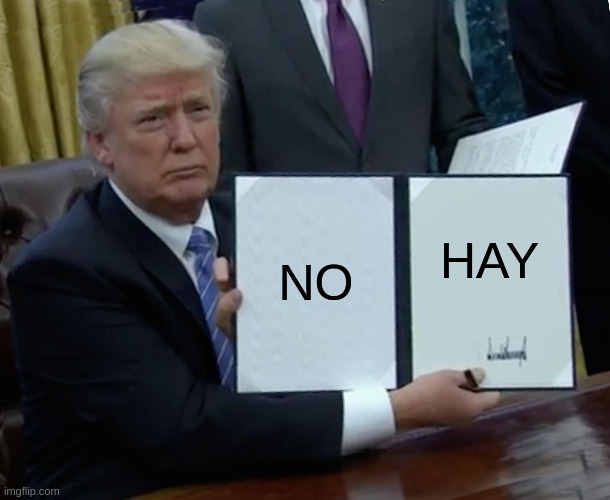
\includegraphics[width=\linewidth]{meme.jpg}

\subsection{Entrega i Evaluación}
Para hacer vàlida vuestra participación nos tendreis que entregar el output de vuestro programa con el formato correcto descrito en el apartado anterior. Para comprovar la score de vuestra solución, podeis descargaros y ejecutar el programa que utilizaremos para determinar vuestra score: [LINK A GITHUB]. 
\end{document}